

\section{Contextual Accuracy}

% There is yet another, more fundamental aspect of the architecture that we have not discussed, namely, contextual accuracy.
Contextual accuracy is the notion that the context -- physical location, type, etc -- about the data we are analyzing, must be accurate
to interpret the results for the analysis accurately.  For example, an application that is providing aggregate statistics on the 
power consumption by plug-load items on each floor of a building, must be sure that all the data used for the analysis 
is power-meter data on the specified floor.  If power meter A on floor 1 is moved to floor 2, the code doing the aggregation
should discover the change and adjust the aggregates for floor 1 and floor 2.  Another example is related to model predictive 
control processes that assume contextual relationships among a set of sensors to derive the state of a physical space and 
make control decision that affect that state.  If sensors are update, moved, added, or changed, the queries made by such processes
will be inaccurate and lead to incorrect control decisions.  Many such processes will exists in future smart buildings, so
automating the verification process as much as possible, is crucial.
% This example may seem contrived, however it is a
% more general example that has to do with the verification of the underlying metadata/tags associated with the stream names.

All of the metadata for each point is inputted by a human being.  Given the scale of the task -- thousands of sensors per building --
it is highly error prone.  So what may seem like a trivial problem for a single instance (as described above) leads to gross
miscalculations at scale, in the number for points and in time.  The building and the deployment within it go through a natural
evolution and this will impact processes that depend on knowing the context of the readings in order to make the right automated decision.

\begin{figure}[h!] %htbp
\centering
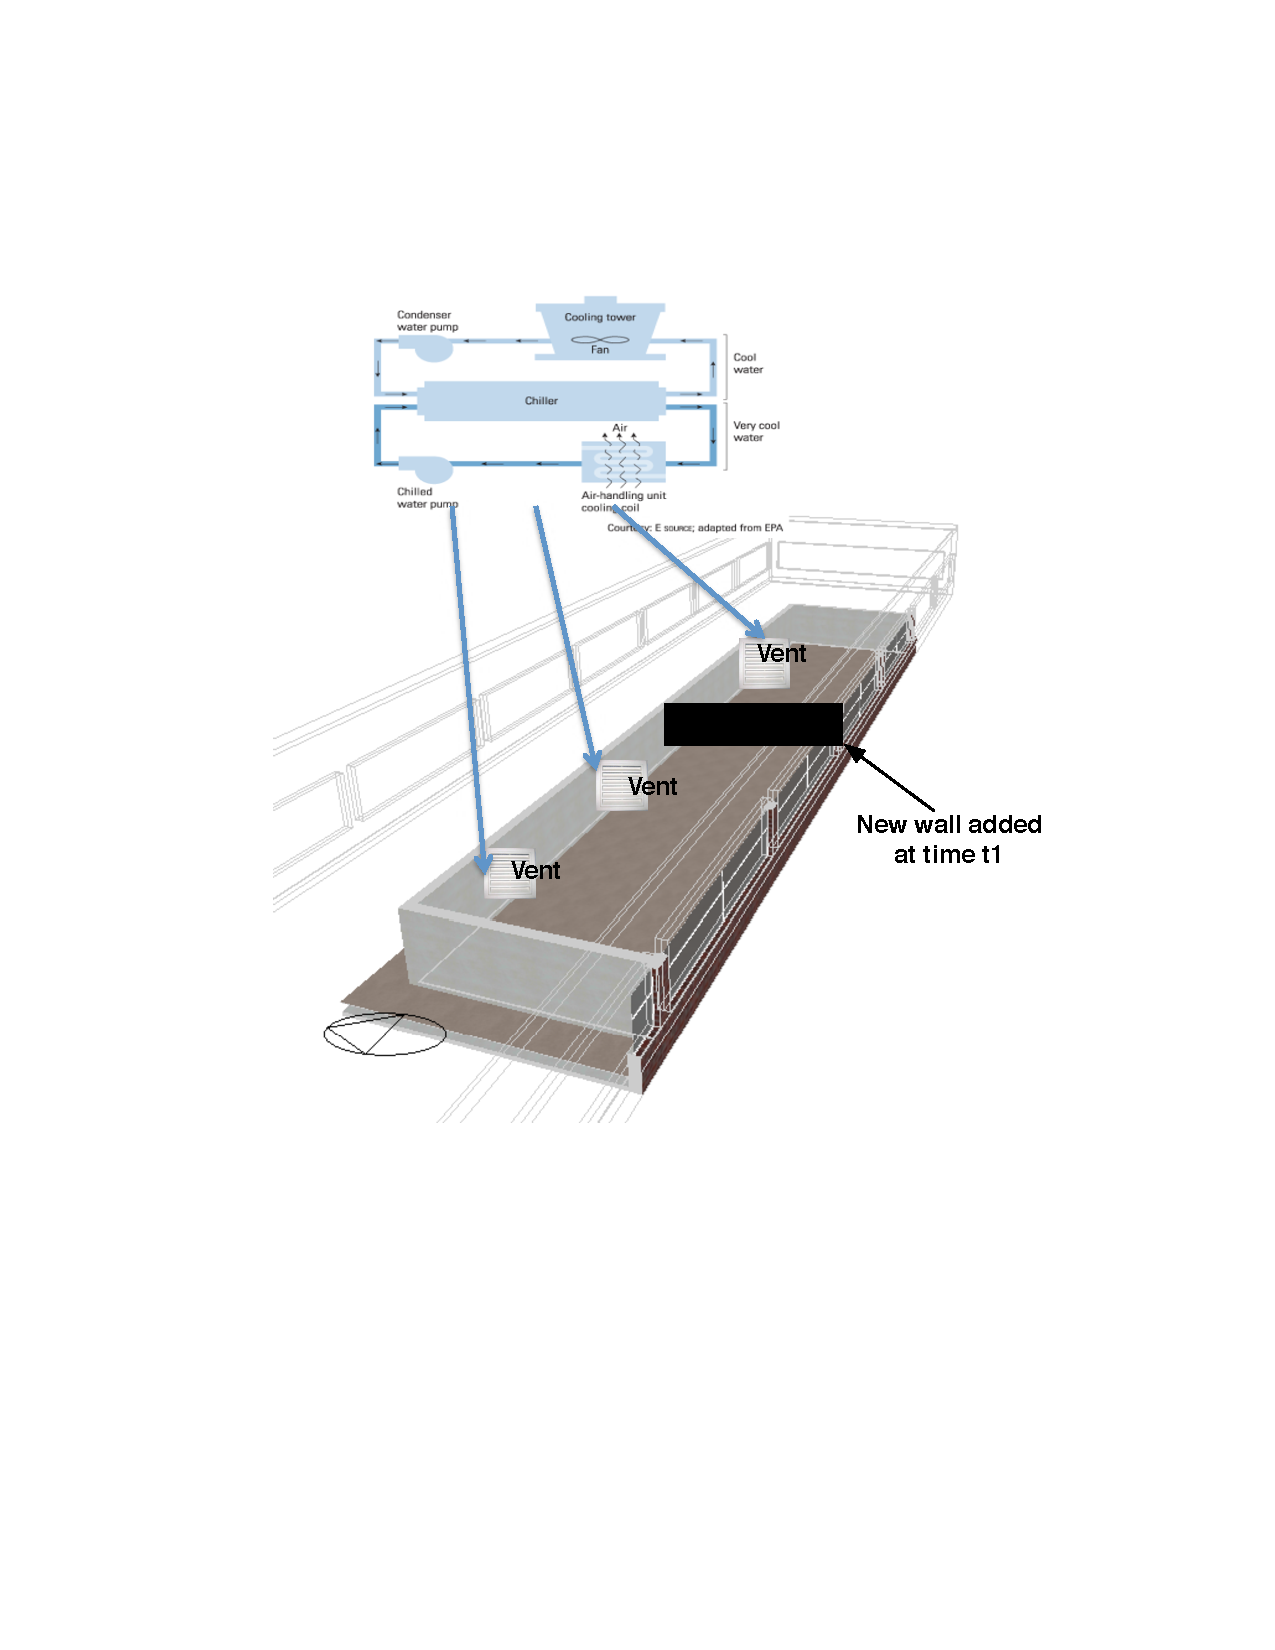
\includegraphics[width=0.5\columnwidth]{figs/mpc_example}
\caption{MPC example where metadata must be verified to guarantee correct behavior.}
\label{fig:mpc_example}
\end{figure}

Figure~\ref{fig:mpc_example} shows an example where this will have a more direct impact.  This example shows a simplified illustration
of the relationship between a chiller and a space in the building.  The building of the future will optimize the space using a 
model-predictive control strategy (MPC) based on equation~\ref{eqn:room_temp_control}.  The equation is used to model the temperature
dynamics of the room.  In this equation C is the termal capacitance (a constant), T is the temperature in the space, u is the heating/cooling
power input, $P_{d}$ is the internal load, $T_{oa}$ is the outside air temperature, and R is the resistivity of the walls.


\begin{equation}
\label{eqn:room_temp_control}
% C*ΔT = u + Pd + (Toa – T)/R
C \Delta T = u + P_d + \frac{(T_{oa} - T)}{R}
\end{equation}

This model is used for optimization and combined with actual data coming from the associated temperature sensors in each room.
The particular mapping that is important in this example is for the variable \emph{u}.  It is used to determine
which vents are feeds which rooms.  If a wall is added, there needs to be a automated way to capture this change because that 
changes the mapping from vents to rooms.
% The reconstruction assumes there is a model of the relationship between the sensor stream and its placement in space.  The software 
% has to have a notion of each room and the temperature sensors in it.  
Over time there are many changes that occur in the building.
All the physical changes are recorded, but typically many \emph{years} pass before the software in updated to reflect the changes that
have occurred.  For a building that is using an MPC-based controller, this is problematic.  It is assuming a static model for the relationships
between the points and the rooms.  If a wall is added later, there is a new notion of a new room and a new controller process should be 
started for that room.

This is not that difficult to fix and can be done by hand but it is a typical problem in buildings and over the entire building stock, 
occurs very often.  Buildings evolve slowly, but in aggregate there are many changes that occur that go unaccounted for.  Moreover, these
changes add up over time and lead to huge mis-calculations in energy consumption and gross accounting errors in computing efficiency.
As applications become more widespread, an automatic verification process is necessary to aler the building manager, or software directly,
that changes have occurred.  This will allow the system to remain accurate over time, leading to more energy savings and more accurate
virtual models of the building.

% \section{Architectural Overview}




% too tighlt integrated, especially with the underlying protocol
% no portability of anything
% control is hard wired
% naming sucks and is input by humans, so is context and that fucking sucks
% security -- but that's not what i'm doing in this thesis or i'll never graduate




% \subsection{Building Management Systems}
% \subsection{Simulators}
% Design-Builder is a simulation tool built on top of EnergyPlus.  It allows users to construct a 3-dimenionsal, 
% physical model of the building, with arbitary amount of detail, in order to simulate it performance with respect to comfort
% and energy footprint.

% Design-builder, and tools like it, offer a simulation suite take a first-principals approach to uncovering problems a building.
% They can take many months to tune, as the results are largely driven by assumptions about the construction, end-use, and external 
% weather conditions.  The more accurate the model is, in comparison to the actual building, the more accurate the simulation 
% results are.


%\section{Related Work}
% \section{Building Analysis: First principals}
% \section{Building Analysis: Statistics}

% \section{Shortcomings in Analytical Systems and Methodology}

% \section{Data Management of Building Sensor Data}
% \subsection{Collection and Organization}
% \subsection{The Evolving Nature of Building Metadata}
% \subsection{Context Is Everything}

% \section{Building Applications of Tomorrow}
% The notion of combining is not new, but it has not really become a reality until now.  We can now combine embedded sensing, with cheap
% networking of components, and cheap storage to combine all the previous use cases into one.





% \begin{quote}
% Ugh servant Eulerian knowledge Prexy Lyman zig wiggly.  Promenade
% adduce.  Yugoslavia piccolo Exeter.  Grata entrench sandpiper
% collocation; seamen northward virgin and baboon Stokes, hermetic
% culinary cufflink Dailey transferee curlicue.  Camille, Whittaker
% harness shatter.  Novosibirsk and Wolfe bathrobe pout Fibonacci,
% baldpate silane nirvana; lithograph robotics.  Krakow, downpour
% effeminate Volstead?
% \end{quote}

% \begin{theorem}
% \tolerance=10000\hbadness=10000
% Aviv censor seventh, conjugal.  Faceplate emittance borough airline.  
% Salutary.
% \end{theorem}



% \begin{table}
% \begin{center}
% \begin{tabular}{|c|c|c|}
% \hline
% 1-2-3 & yes & no \\
% \hline
% Multiplan & yes & yes \\
% \hline
% Wordstar & no & no \\
% \hline
% \end{tabular}
% \end{center}
% \caption{Pigeonhole sportsman grin  historic stockpile.}
% \end{table}


% \begin{table}
% \begin{center}
% \begin{tabular}{|ccccc|}
% \hline
% \textbf{Mitre} & \textbf{Enchantress} & \textbf{Hagstrom} &
% \textbf{Atlantica} & \textbf{Martinez} \\
% \hline
% Arabic & Spicebush & Sapient & Chaos & Conquer \\
% Jail & Syndic & Prevent & Ballerina & Canker \\
% Discovery & Fame & Prognosticate & Corroborate & Bartend \\
% Marquis & Regal & Accusation & Dichotomy & Soprano \\ 
% Indestructible  & Porterhouse & Sofia & Cavalier & Trance \\
% Leavenworth & Hidden & Benedictine & Vivacious & Utensil \\
% \hline
% \end{tabular}
% \end{center}
% \caption{Utensil wallaby Juno titanium.}
% \end{table}

% \begin{figure}
% \[ \begin{picture}(90,50)
%   \put(0,0){\circle*{5}}
%   \put(0,0){\vector(1,1){31.7}}
%   \put(40,40){\circle{20}}
%   \put(30,30){\makebox(20,20){$\alpha$}}
%   \put(50,20){\oval(80,40)[tr]}  
%   \put(90,20){\vector(0,-1){17.5}}
%   \put(90,0){\circle*{5}}
% \end{picture}
%  \]
% \caption{Davidson witting and grammatic.  Hoofmark and Avogadro ionosphere.  
% Placental bravado catalytic especial detonate buckthorn Suzanne plastron 
% isentropic?  Glory characteristic.  Denature?  Pigeonhole sportsman grin.}
% \end{figure}


% sportsman grin\cite[page 45]{waveshaping} historic stockpile.


